% type de document
\documentclass[11pt]{article}

% Inclusion des packages :
\usepackage{geometry}	% Permet de régler les marges
\usepackage{listings}	% Permet d'inclure des listing de code.
\usepackage[utf8]{inputenc}	% Permet de taper directement les caractères accentués
\usepackage[french]{babel}	% Pries en charge du français.
\usepackage{graphicx}	% Permet d'inclure des images bitmap (jpg,gif,png) ou vectorielles (pdf)


% Instruction poru le package geometry
\geometry{hmargin=1.5cm, vmargin=1.5cm }

% mode de présentation par défaut du package listing
\lstset{language=Java, numbers=left, tabsize=2, frame=single, breaklines=true, numberstyle=\tiny\ttfamily, framexleftmargin=13mm, xleftmargin=12mm}

\author{A. Turing, M. Minsky}
\title{Notre beau compte-rendu de TP}

% Début du corps du document
\begin{document}

% Provoque l'affichage de l'en-tête :
\maketitle

\section{Introduction}
Babla

\section{Exercice 1}

Blabla

\subsection{Nos fonctions}
%
Blabla On rappelle que $e = mc^2$ % un seul $, equation en ligne
et que
% On peut faire facilement des super formules :
$$Z=\sum_{i=1}^{i\leq n} \sqrt[3]{x^{i-1}} f(x_i)$$
% De manière générale, ce qui est entre crochet peut-être omis en latex (options).

Du code :
\begin{lstlisting}
class LabelledData {
	private int cls;
	private byte[] glyph;
	
	public LabelledData(int cls, byte[] glyph) { this.cls=cls; this.glyph = glyph; }
	int getCls() { return cls; }
	byte[] getGlyph() {return glyph; }
}
\end{lstlisting}
Fichier externe :
\lstinputlisting{lab.java}

\subsection{Nos résultats expérimentaux}
ça marche !
On peut inclure une figure en y faisant référence : nous obtenons une belle sinsoïde (voir Figure~\ref{sinu}).

\begin{figure}
\center{
	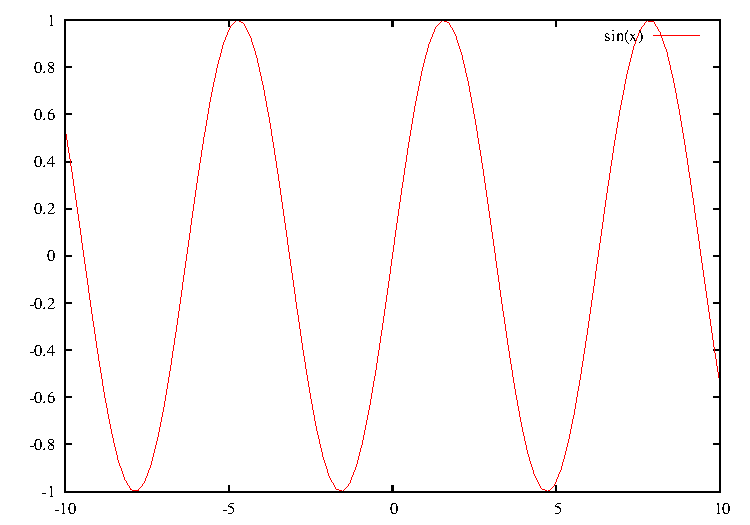
\includegraphics[scale=0.75]{sin.pdf}
}
\caption{Une belle sinusoïde\label{sinu}}	% Legende + étiquette
\end{figure}

\section{Exercice 2}
Ipsum Lorem...

\section{conclusion}
Nous avons tout compris.


\end{document}
